\documentclass[12pt]{article}

% Packages
\usepackage[utf8]{inputenc}
\usepackage{amsmath}
\usepackage{amssymb}
\usepackage{graphicx}
\usepackage{hyperref}
\usepackage{geometry}
\usepackage{float}

% remove the indent at the beginning of a paragraph:
\setlength{\parindent}{0pt}

% Line spacing
\renewcommand{\baselinestretch}{1}

% distance between new paragraphs:
\setlength{\parskip}{0.5em}

% Title design:
\usepackage{titling}
\pretitle{\begin{center}\LARGE\bfseries}
\posttitle{\par\end{center}\vspace{-0.5em}}
\preauthor{\begin{center}\large}
\postauthor{\par\end{center}\vspace{-2em}}
\predate{\begin{center}\large}
\postdate{\par\end{center}\vspace{-1em}}


% Geometry settings
\geometry{
    a4paper,
    total={170mm,257mm},
    left=20mm,
    right=20mm,
    top=20mm,
    bottom=20mm,
}

% Set the figure counter to reset within subsections
\counterwithin{figure}{subsection}

% Document
\begin{document}

% Title Page
\title{Homework 1: Vector Search}
\author{Naomi Derel 325324994, Gili Cohen 326280815, Renana Shachak 213920010}
\date{02.07.2024}
\maketitle

% % Table of Contents
% \tableofcontents
% \newpage

% Sections
\section{Faiss}

With permission from the course staff, we kept our answers for the original question and not the updated requirements as we finished it prior to the update.

\subsection{Running Times}

\begin{figure}[H]
    \centering
    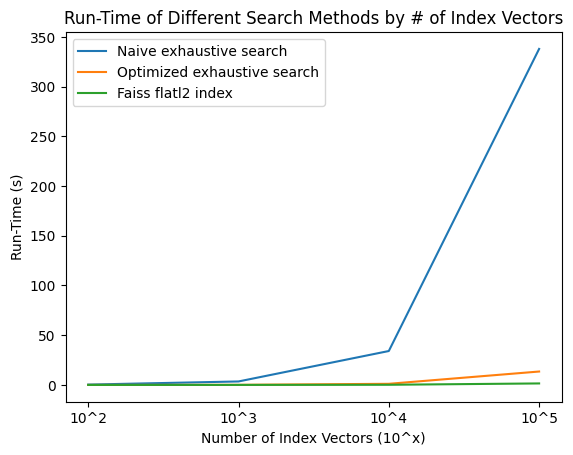
\includegraphics[width=0.8\textwidth]{images/1_1_1.png}
    \caption{Running times by Number of Index Vectors}
\end{figure}

\begin{figure}[H]
    \centering
    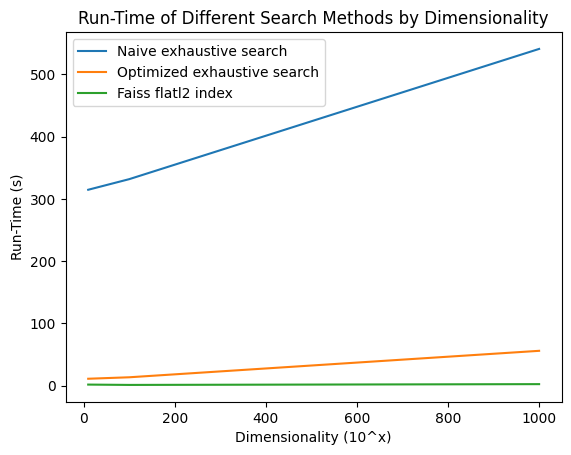
\includegraphics[width=0.8\textwidth]{images/1_1_2.png}
    \caption{Running times by Dimentionality}
\end{figure}

\subsection{Faiss LSH}

\begin{figure}[H]
    \centering
    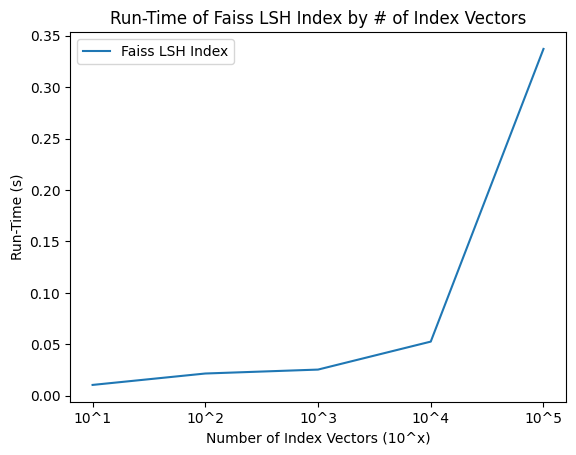
\includegraphics[width=0.8\textwidth]{images/1_2_1.png}
    \caption{Running times by Number of Index Vectors}
\end{figure}

\begin{figure}[H]
    \centering
    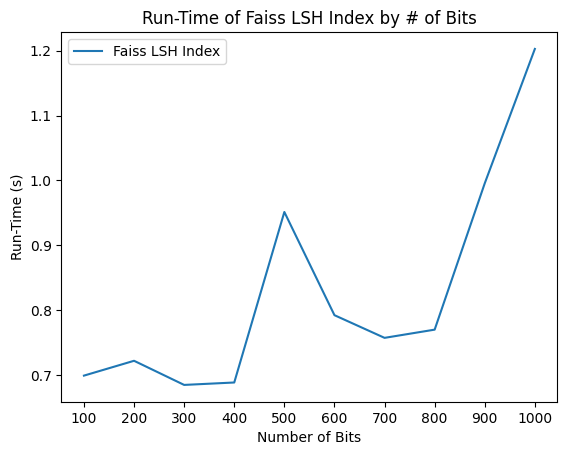
\includegraphics[width=0.8\textwidth]{images/1_2_2.png}
    \caption{Running times by Number of Bits}
\end{figure}

\begin{figure}[H]
    \centering
    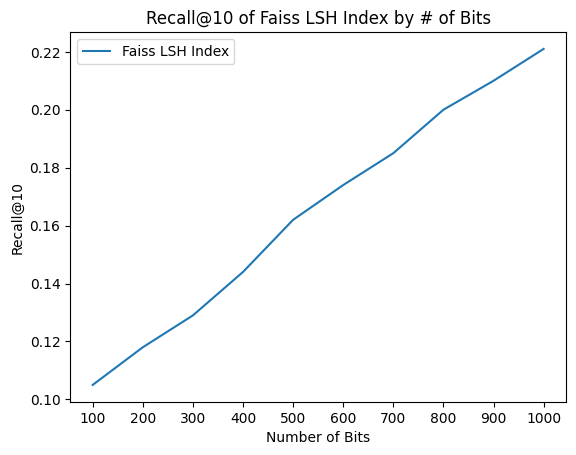
\includegraphics[width=0.8\textwidth]{images/1_2_3.png}
    \caption{$Recall@10$ by Number of Bits}
\end{figure}

\newpage

\section{Implementing an Index}

\subsection{LSH vs. Native Exhaustive Search}

\begin{enumerate}
    \item Running time of the \texttt{semi optimized exhaustive search} function was: \textbf{4.14 seconds}.
    \item Running time of building the LSH index was: \textbf{0.62 seconds}.
    \item Running time of LSH search over query vectors was: \textbf{0.13 seconds}.
    \item $Recall@10$ for the LSH index was: \textbf{0.138}.
\end{enumerate}

\subsection{Custom Indexing Algorithm}

\subsubsection*{Implementation Description}

For our solution, we decided to implement an index based on the HNSW algorithm we saw in the lecture. 
Our intuition for this choice comes from the assumption that the HNSW is a very fast algorithm based on the skip-list data structure, and yet it is more accurate than the LSH algorithm.

We supported this intuition by testing the implementation of the HNSW algorithm in the Faiss library, and found that an ideal implementation can reach the 0.8 recall@10 mark in a very short time.

For our implementation, we...

\subsubsection*{Performance Measures}

\begin{itemize}
    \item \textbf{creating custom indexing algorithm:} x seconds, half the time of section 2.1.2
    \item \textbf{searching with custom indexing algorithm:} x seconds, a third of the time of section 2.1.3
    \item \textbf{recall@10 for custom indexing algorithm:} x, at least 0.8
\end{itemize}



\newpage

\section{Pinecone VectorDB and RAG}

\subsection{Dataset Selection}

We opted to use the Stanford Question Answering Dataset (SQuAD) as the dataset for this task. 
It consists of questions posed by crowdworkers on a set of Wikipedia articles, with corresponding reading passages.
In total, SQuAD 1.1 contains 100,000+ question-answer pairs on 500+ articles.

The segments of contexts are repeated across questions, and after eliminating duplicates, we are left with 20,958 unique contexts.

The answers for the questions are usually short, precise answers that can be found in the context, which makes them potentially easier to compare with the generated answer. However, there are also some questions that do not have an answer in the context.

\subsection{Standard Model Evaluation}

The standard QA model from cohere may fall short in answering factual questions in specific domains it might have not been exposed to enough. We present a few anecdotal examples of such cases:

\begin{enumerate}
    \item \textbf{How many student news papers are found at Notre Dame?}
    The correct answer is 3, but the model answered: "There are two student newspapers at the University of Notre Dame: 1. The Observer: This is the main student newspaper on campus and is published daily during the academic year. It covers a wide range of topics, including news, sports, opinion, and entertainment. 2. Irish Informer: This is a newer, independent student-run newspaper that was founded in 2013. It publishes weekly and focuses on providing an alternative perspective on campus news and events. Both newspapers are valuable sources of information and showcase the diverse talents and interests of the student body at Notre Dame."
    
    This is an example of a factual error based on lack of accurate or current information.
    
    \item \textbf{q2}

\end{enumerate}


\subsection{RAG Pipeline}

\subsection{Insights}

% % Bibliography
% \newpage
% \begin{thebibliography}{99}
%     \bibitem{ref1} Author, \emph{Title}, Publisher, Year.
%     \bibitem{ref2} Author, \emph{Title}, Publisher, Year.
%     % Add more references as needed
% \end{thebibliography}

\end{document}